\documentclass[11pt,a5paper]{article}
\usepackage[utf8]{inputenc}
\usepackage[english]{babel}
\usepackage{amsmath}
\usepackage{graphicx}
\usepackage{amsthm}
\usepackage{amsfonts}
\usepackage[margin=0.47in]{geometry}

\newtheorem{theorem}{}
\newtheorem{definition}{Definition}
\newtheorem{exercise}{Exercise}
\newtheorem{example}{Example}
\newtheorem{problem}{Problem}
\newtheorem*{corollary}{Corollary}

\makeatletter
\newenvironment{chapquote}[2][2em]
  {\setlength{\@tempdima}{#1}%
   \def\chapquote@author{#2}%
   \parshape 1 \@tempdima \dimexpr\textwidth-2\@tempdima\relax%
   \itshape}
  {\par\normalfont\hfill--\ \chapquote@author\hspace*{\@tempdima}\par\bigskip}
\makeatother

\title{\textbf{Combinatorics}}
\date{Week 6}
\author{Ivan Lau\\}
\begin{document}
\maketitle


\section{Two fundamental counting principles}

\begin{definition}[Addition principle, \textbf{AP}]
If we have $m$ ways of doing something and $n$ ways of doing another thing; and we cannot do both at the same time, then there are $m+n$ ways to choose one of the actions.
\end{definition}

\begin{definition}[Multiplication principle, \textbf{MP}]
If there are $m$ ways of doing something and n ways of doing another thing, then there are $m \times n$ ways of performing both actions.
\end{definition}

\begin{example} Find the number of ordered pairs $(x,y)$ of integers such that $x^2+y^2 \le 5$.\\
\textit{Solution}: We divide the problem into $6$ disjoint cases: $x^2+y^2 = 0,1,…,5$. It can be checked that the number of ways are respectively $1,4,4,0,4,8$. By AP, the number of ordered pairs is $21$.
\end{example}

\begin{example} Find the number of positive divisors of $60$. \\
\textit{Solution}: Note that $60$ has a unique prime factorisation of $2^2 \times 3^1 \times 5^1$. For all positive integers $m$, they are a divisor of $60$ iff $m$ is of the form $2^a \times 3^b \times 5^c$, where $a \in \{0,1,2\}$, $b \in \{0,1\}$ and $c \in \{0,1\}$. By MP, the number of divisors is $3 \times 2 \times 2 = 12$.
\end{example}

\noindent Both AP and MP seem trivial, and this could be the reason why they are often neglected. Actually, they are very fundamental in solving counting problems. As we shall encounter later, given counting problem, no matter how complicated it is, it can always be decomposed into simpler sub-problems that can be solved using AP and/or MP.

\begin{example} Let $S = \{(a,b,c) | a,b,c \in \{1,2,…100\}; a<b; a<c\}$.  Find n(S). \\
\textit{Solution}: Categorise the elements of $S$ by considering $a = 1,2,…,99$.  For $a = k \in \{1,2,…,99\}$, the number of choices for $b$ and $c$ are respectively $(100-k)$.The number of possible triplets $(k,b,c)$ is then $(100-k)^2$ by MP. Since $k$ takes on values $1,2,…,99$, by applying AP, \[n(S)= \sum_1^{99}{k^2} = 328350\].
\end{example}

\section{Permutations, Combinations}

\begin{definition}[Permutations]
Given a set of $n$ distinct objects, for $0 \le r \le n$, $P_r^n$ is number of ways of arranging any $r$ of the objects in a row. This is a derivation of MP where first object has $n$ choices, second object has $(n-1)$ choices, …, and $r$-th object has $(n-r+1)$ choices.
\[P_r^n=n(n-1)(n-2)\cdots(n-r+1)\]
Multiplying by $\frac{(n-r)!}{(n-r)!}$, we get $P_r^n = \frac{n!}{(n-r)!}$.
\end{definition}

\begin{definition}[Combinations]
Given a set of $n$ distinct objects, for $0 \le r \le n$, $n \choose r$ is number of ways of choosing any $r$ of the objects. How are combinations related to permutations? Note that we can get $P_r^n$ by first choosing a subset of size r and arrange the r obejcts. By MP, $P_r^n = {n \choose r} \cdot r!$. Rearranging, we get \[{n \choose r} = P_r^n r!= \frac{n!}{r!(n-r)!}\]
\end{definition}

\begin{definition}[Principle of Complementation, \textbf{CP}]
If $A$ is a subset of finite universal set $U$, then $n(\overline{A}) = n(U) - n(A)$
\end{definition}

\begin{example}
How many ways can $8$ people sit in a line if Alice and Bob are not adjacent? \\
\textit{Solution 1 (CP way)}: Subtract the number of ways the $8$ people can be seated with Alice and Bob adjacent from the total number of ways the $8$ people can sit in a line. We get $8!- 2 \times 7! = 6 \times 7!$ ways. \\
\textit{Solution 2}: Arrange the other $6$ people and Alice in a straight line. Bob then have $6$ out of $8$ spots (except the front and back of Alice) for him to choose where to sit. By MP, we get $7! \times 6$ ways.   
\end{example}

\noindent Different approach, same answer. Interesting huh. Indeed this is the fun part of combinatorics or perhaps mathematics. Even though beauty is in the eye of beholder, some approaches are objectively more elegant than the other approaches. Let's now dive in into problems and try to come out with as many approaches as you can and compare it with what your friends got!

\subsection*{Problems}

\begin{problem}
Prove that ${n \choose r} = {n \choose n - r}$.
\end{problem}

\begin{problem}
How many ways are there to split a dozen people into 3 teams, where each team has 4 people?
\end{problem}

\begin{problem}
Prove that $n{n-1 \choose k-1}= k{n \choose k}$.
\end{problem}

\begin{problem}
See that there are ${n+r-1 \choose r}$ ways to choose $r$ items from $n$ with repetition allowed.
\end{problem}

\begin{problem}
How many solutions are there for $a_1 + a_2 + \dots + a_n = s$, for given positive integer $s$, where all $a_i$ are nonnegative integers?
\end{problem}

\begin{problem}
Interpret $\sum_{i=1}^{n} i = {n+1 \choose 2}$.
\end{problem}

\begin{problem}
Prove that ${n \choose r} = {n - 2 \choose r - 2} + 2{n - 2 \choose r - 1} + {n - 2 \choose r}$.
\end{problem}

\begin{problem}
Let $A$ be a \textit{2n}-element set with $n \ge 1$. Find the number of different pairings of $A$.
\end{problem}

\begin{problem}
Prove that $\sum_{i=1}^{n-1} (i - 1)i(n-i-1) = 2{n \choose 4}$.
\end{problem}

\begin{problem}
Show that $49$ divides $8^n - 7n - 1$ for all $n \ge 0$.
\end{problem}

\begin{problem}
See that $\sum_{i=1}^n i^2 = 2 {n+1 \choose 3} + {n+1\choose 2}$.
\end{problem}

\begin{problem}
Let $X_n$ be number of words of length $n$ from letters A and B not containing sequence "ABABA" or "BABAB" and $Y_n$ number of words of length $n$ from letters A and B not containing 5 same letters in a row. See that $X_n = Y_n$.
\end{problem}

\begin{problem}
Show that ${n+1 \choose 2}^2 = (\sum_{i=1}^n i^3) = 6{n+1 \choose 4} + 6{n+1 \choose 3} + {n+1 \choose 2}$
\end{problem}

\begin{problem}
See that number of parallelograms in a triangular grid of size $n$ is $3{n \choose 4}$.
\end{problem}
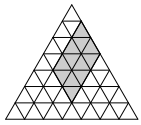
\includegraphics[scale=0.8]{triangle}

\begin{problem}
Let $a_1 + a_2 + \dots + a_n = s$ with all $a_i$ and $s$ being natural numbers. Show that the sum of all possible $a_1 \cdot a_2 \cdots a_n = {s + n - 1 \choose 2n - 1}$
\end{problem}

\begin{problem}
Show that $\sum_{k=0}^n {2k \choose k}{2(n-k)\choose n-k} = 2^{2n}$.
\end{problem}

\end{document}

